\subsection{Точки Лагранжа}

\term{Точки Лагранжа}~--- точки во вращающейся системе из двух массивных тел,
\begin{wrapfigure}[14]{l}{0.48\tw}
	\centering
	\vspace{-.5pc}
	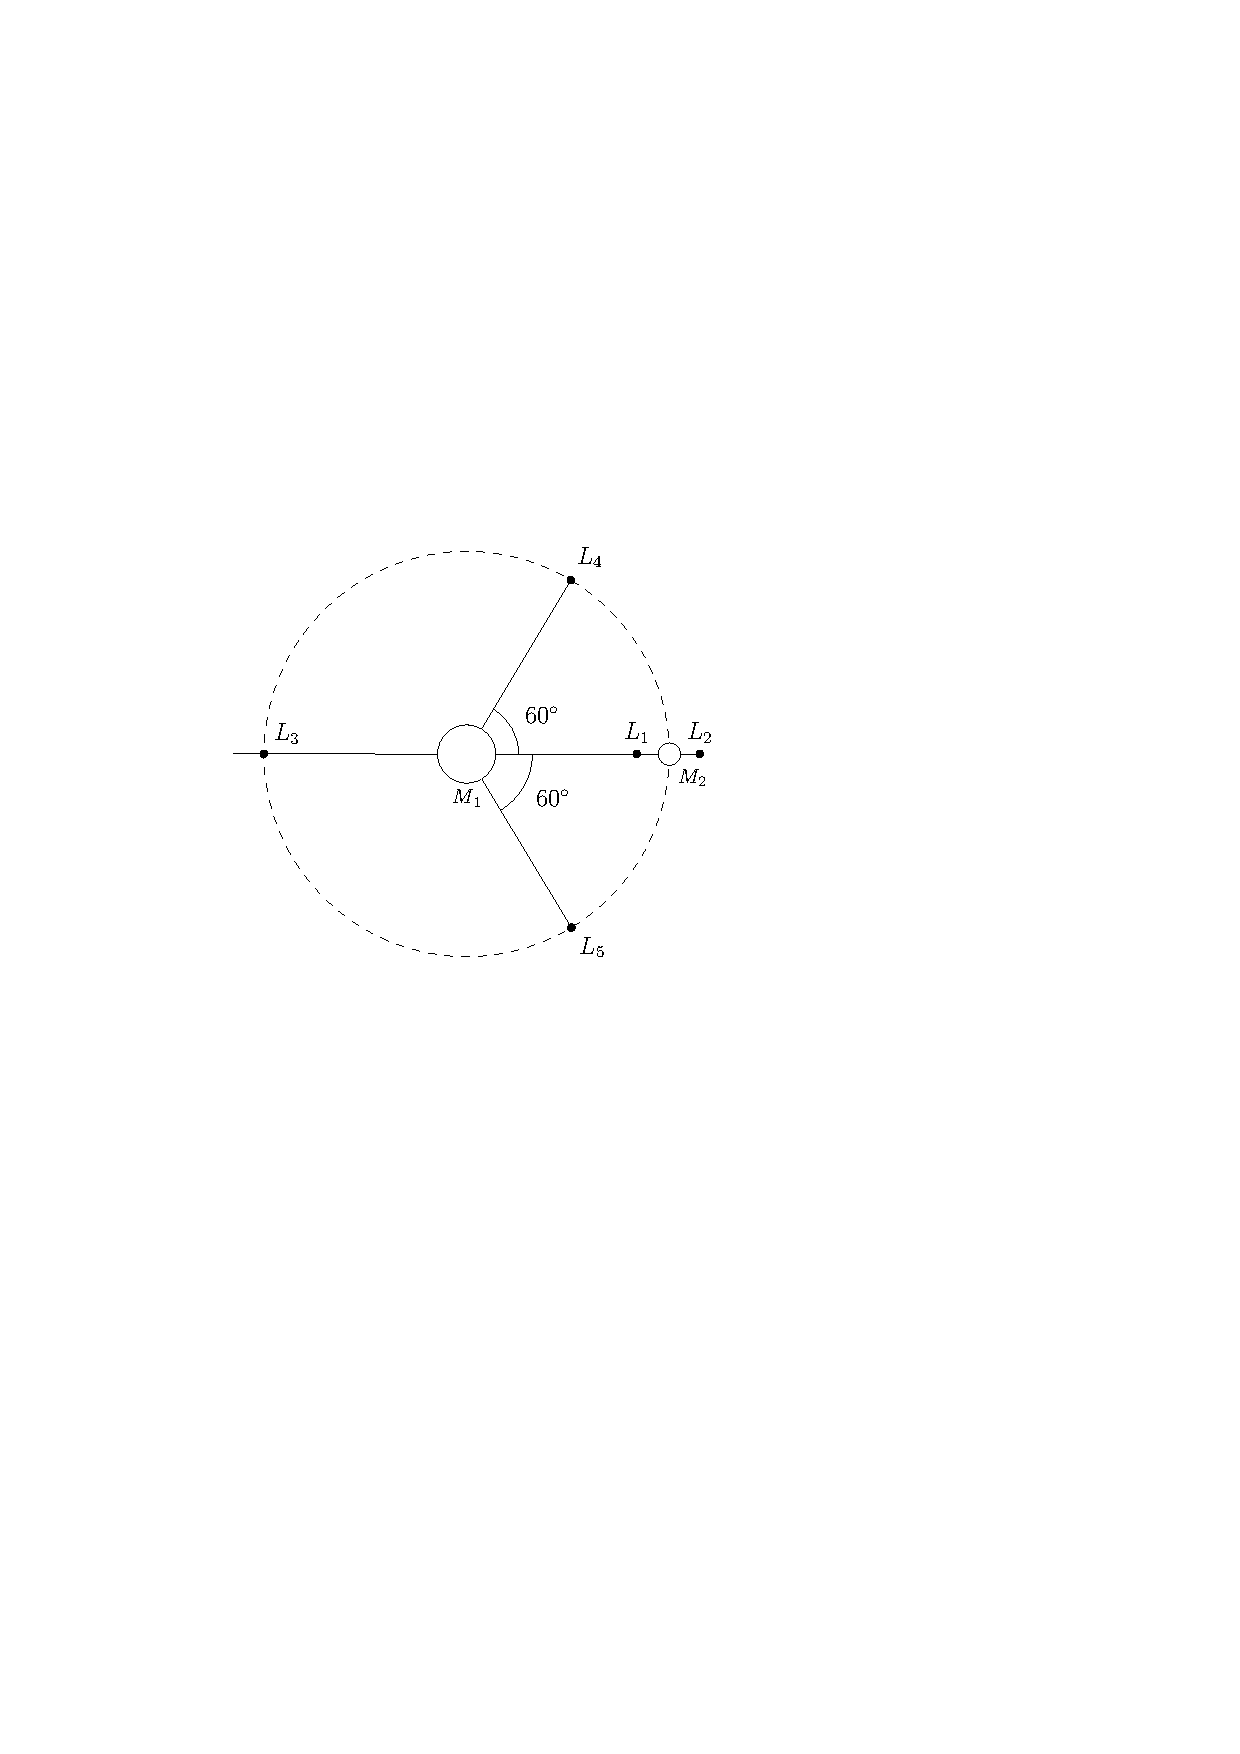
\includegraphics[width = .48\tw]{lagr-points}
	\captionof{figure}{Точки Лагранжа}
	\label{pic:larg-points-1}	
\end{wrapfigure}
в которых третье тело с пренебрежимо 
малой массой, не испытывающее воздействие никаких 
других сил, кроме гравитационных со стороны двух 
первых тел, может оставаться неподвижным относительно 
этих тел. В этих точках гравитационные силы, 
действующие на малое тело, уравновешиваются силами инерции.

Точки $L_1$, $L_2$ и $L_3$ лежат на одной прямой, 
соединяющей два массивных тела (см.~Рис.\,\ref{pic:larg-points-1}). 
В системе Солнце\,--\,Земля точка $L_1$ находится между Землёй и 
Солнцем, $L_2$~--- с противоположной стороны от Земли, а точка 
$L_3$ располагается за Солнцем. Точки $L_4$ и $L_5$ 
образуют равносторонние треугольники с массивными телами.

%Для расстояний до точек $L_1$, $L_2$ и $L_3$ от 
%центра масс системы справедливы следующие выражения:
%\begin{equation}r_1=R\left(1-\sqrt[3]{\frac{\alpha}
%{3}}\right), \quad r_2=R\left(1+\sqrt[3]{\frac{\alpha}
%{3}}\right), \quad r_3=R\left(1+\frac{5}{12}\alpha\right),
%\end{equation}
%где $\alpha=M_2 / (M_1 + M_2)$, $R$~--- расстояние между 
%телами, $M_1$ --- масса более массивного тела, $M_2$
% --- масса второго тела.
%
%Если $M_2 \ll M_1$, то точки $L_1$ и $L_2$ находятся 
%примерно на одинаковом расстоянии от тела $M_2$, равном
%\begin{equation}
%r\approx R\sqrt[3]{\frac{M_2}{3M_1}}.
%\end{equation}



\begin{wrapfigure}[5]{r}{0.45\tw}
	\centering
	\vspace{-.5pc}
	\begin{tikzpicture}[scale = 0.66]
			\small
			%
			\draw (5, 0) node [anchor= south] {$M_2$};
			\draw (-1, 0) node [anchor= south] {$M_1$};
			\draw (4, 0) node [anchor= south] {$L_1$};
			\draw (0, 0) node [anchor= south] {ц.м.};
			%
			\draw [dashed] (-1, 0) -- (5, 0);
			%
			\draw[fill=white] (-1, 0) circle (0.05); %%% 1
			\draw[fill=white] (5, 0) circle (0.05); %%% 2
			\draw[fill=white] (4, 0) circle (0.05); %%% 3
			\draw[fill=white] (0, 0) circle (0.05); %%% ЦМ
			%
			\draw [latex-latex] (4, -- -.3) -- (5, -.3);
			\draw (4.5, -.3) node [anchor= north] {$r$};
			%
			\draw [latex-latex] (-1, -.3) -- (4, -.3);
			\draw (1.5, -.3) node [anchor= north] {$R - r$};
		\end{tikzpicture}
	\captionof{figure}{Расположение точки $L_1$}
%	\label{pic:larg-points}	
\end{wrapfigure}\change{Получим выражения для расстояний от центра масс системы до точек Лагранжа. Проще всего это сделать для точек $L_1$ и $L_2$. Пусть $R$~--- расстояние между телами, $M_1$ и $M_2$~--- их массы. Будем искать расстояние~$r$ до точки $L_1$ от тела $M_2$.
}



\change{Из уравнения моментов сил тело с массой $M_2$ находится на расстоянии $\beta R$ от центра масс, где $\beta \equiv M_1 / (M_1 + M_2)$. Тело с массой $M_1$, соответственно, --- на расстоянии $\alpha R$, где $\alpha \equiv M_2 / (M_1 + M_1)$. Легко видеть, что $\alpha + \beta = 1$, данный факт пригодится ниже.} 

\change{Запишем уравнение баланса сил, действующих на пробное тело в точке~$L_1$:
\begin{equation}
	\frac{GM_1 m}{(R - r)^2} = \frac{G M_2 m}{r^2} + m \omega^2 \left(R \cdot \frac{M_1}{M_1 + M_2} - r \right),
	\label{eq:lagrange-1}
\end{equation}
где $\omega$~--- угловая скорость вращения системы вокруг центра масс, выразим её из обобщенного третьего закона Кеплера:
\begin{equation*}
	\frac{G \left(M_1 + M_2 \right)}{R^3} = \frac{4 \pi^2}{T^2} = \omega^2.
\end{equation*}
Подставим угловую скорость в \eqref{eq:lagrange-1}:
\begin{gather*}
	\frac{GM_1 m}{(R - r)^2} = \frac{G M_2 m}{r^2} + m \frac{G \left(M_1 + M_2 \right)}{R^3} \left(R \cdot \frac{M_1}{M_1 + M_2} - r \right),\\
	\frac{M_1}{(R - r)^2} = \frac{M_2}{r^2} + \frac{M_1 + M_2}{R^3} \left(R \cdot\frac{M_1}{M_1 + M_2} - r \right),\\
	\frac{M_1}{(R - r)^2} = \frac{M_2}{r^2} + \frac{M_1}{R^2} - \frac{\left(M_1 + M_2 \right)}{R^2} \cdot \frac{r}{R}.
\end{gather*}
Рассмотрим случай $M_2 \ll M_1$, тогда $r \ll R$, следовательно
\begin{gather*}
	\frac{M_1}{R^2} \left(1 + \frac{2r}{R} + o\left(\frac{r}{R}\right) \right) = \frac{M_2}{r^2} + \frac{M_1}{R^2} - \frac{\left(M_1 + M_2 \right)}{R^2} \cdot \frac{r}{R},\\
	\frac{M_1}{R^2} \left( 1 + \frac{2r}{R} - 1 + \frac{r}{R}  + o\left(\frac{r}{R}\right) \right) = M_2 \left( \frac{1}{r^2} - \frac{r}{R^3} \right), \\
	\frac{M_1}{R^2} \left( \frac{3r}{R} + o\left(\frac{r}{R}\right) \right) = 
	% \frac{M_2}{r^2} \left( 1 - \frac{r^3}{R^3} \right) = 
	\frac{M_2}{r^2} \left( 1 +  o\left(\frac{r}{R}\right)  \right),\\
	\frac{M_1}{R^2} \cdot \frac{3r}{R} \simeq \frac{M_2}{r^2} \quad \Rightarrow \quad r \simeq R \sqrt[3]{\frac{M_2}{3M_1}}.
\end{gather*}
Заметим, что в уравнение для точки $L_2$ с точностью до знака перед $r$ совпадает с \eqref{eq:lagrange-1}. Следовательно, расстояние от центра масс системы до точек $L_1$ и $L_2$ определяются, как 
\begin{equation}
	R_{1,2} = R \left( 1 \mp \sqrt[3]{\frac{M_2}{3M_1}} \right).
\end{equation}
}

\begin{wrapfigure}[5]{r}{0.45\tw}
	\centering
	\vspace{-.5pc}
	\begin{tikzpicture}[scale = 0.66]
			\small
			%
			\draw (3, 0) node [anchor= south] {$M_2$};
			\draw (0, 0) node [anchor= south] {$M_1$};
			\draw (-3, 0) node [anchor= south] {$L_3$};
			\draw (1, 0) node [anchor= south] {ц.м.};
			%
			\draw [dashed] (-3, 0) -- (3, 0);
			%
			\draw[fill=white] (0, 0) circle (0.05); %%% 1
			\draw[fill=white] (3, 0) circle (0.05); %%% 2
			\draw[fill=white] (-3, 0) circle (0.05); %%% 3
			\draw[fill=white] (1, 0) circle (0.05); %%% ЦМ
			%
			\draw [latex-latex] (0, -.3) -- (3, -.3);
			\draw (1.5, -.3) node [anchor= north] {$R$};
			%
			\draw [latex-latex] (-3, -.3) -- (0, -.3);
			\draw (-1.5, -.3) node [anchor= north] {$R - r$};
		\end{tikzpicture}
	\captionof{figure}{Расположение точки $L_3$}
%	\label{pic:larg-points}	
\end{wrapfigure}\change{Найдем теперь расстояние $R_3$ от центра масс до точки $L_3$. Пусть точка $L_3$ находится на расстоянии $R - r$ от тела с массой $M_1$. Будем искать расстояние~$r$. Запишем баланс сил, предварительно сократив на $Gm$: 
\begin{equation}
	\frac{M_1}{(R - r)^2} + \frac{M_2}{(2R - r)^2} =  \frac{M_1 + M_2}{R^3} \left(R - r + R \cdot \frac{M_2}{M_1 + M_2} \right).
	\label{eq:lagrange-2}
\end{equation}
Снова рассмотрим случай $M_2 \ll M_1$, когда $r \ll R$, тогда \eqref{eq:lagrange-2} будет выглядеть, следующий образом:
\begin{gather*}
	\frac{M_1}{R^2} \left(1 + \frac{2r}{R} \right) + \frac{M_2}{4R^2} \left(1 + \frac{r}{R} \right) \simeq \frac{M_1}{R^2} + \frac{M_2}{R^2} - \frac{M_1}{R^2} \cdot \frac{r}{R} - \frac{M_2}{R^2} \cdot \frac{r}{R} + \frac{M_2}{R^2},\\
	\frac{r}{R} \left( \frac{3M_1}{R^2} + \frac{5M_2}{4R^2} \right) \simeq \frac{7M_2}{4R^2} \quad \Rightarrow \quad r \simeq R \cdot \frac{7 M_2}{12 M_1}.
%	\frac{r}{R} \left( 3 + \frac{5M_2}{4M_1} \right) \simeq \frac{7M_2}{4M_1},\\[0.5pc]
\end{gather*}
 Следовательно, расстояние до точки $L_3$ от центра масс системы равно
 \begin{equation}
 	R_3 \simeq R - r + R \cdot \frac{M_2}{M_1} =
% 	R \left(1 - \frac{7 M_2}{12 M_1} + \frac{M_2}{M_1} \right) = 
 	R \left( 1 + \frac{ 5 M_2}{12 M_1} \right). 
 \end{equation}
 }
 
 \change{Остается найти координаты точек Лагранжа $L_4$ и $L_5$. Рассмотрим~Рис.\,\ref{pic:larg-points-2}. Векторы $\vec{r}_1$, $\vec{r}_2$ и $\vec{r}_3$~--- радиус-векторы соответсвенно тела с массой $M_1$, тела с массой $M_2$ и центра масс относительно точки $L_4$. В~силу симметрии  все рассуждения будут верны и для точки $L_5$.Также на рисунке отмечены силы, действующие на тело, располагающееся в точке $L_4$: $\vec{F}_1$~--- сила гравитации от тела с массой $M_1$, $\vec{F}_2$~--- с массой $M_2$, сила инерции $\vec{F}_\text{ц.б.}$~--- центробежная~--- коллинеарна вектору $\vec{r}_3$.
 }
 
 \begin{figure}[h!]
	\begin{subfigure}{0.47\tw}
		\begin{tikzpicture}[scale = 0.66]
			\small
			\draw [-latex] (2, 5.2) -- (5,0);
			\draw [-latex] (2, 5.2) -- (-1,0);
			\draw [-latex] (2, 5.2) -- (0, 0);

			\draw (5, 0) node [anchor= north west] {$M_2$};
			\draw (-0.9, 0) node [anchor= north east] {$M_1$};
			\draw (0, 0) node [anchor= north] {ц.м.};
			\draw (2, 5.2) node [anchor= south east] {$L_4$};
	
			\draw [dashed] (-1, 0) -- (5, 0);
	
			\draw (-.5, 0.87) node [anchor= south east] {$\vec{r}_1$};
			\draw (3.5, 2.6) node [anchor= south west] {$\vec{r}_2$};
			\draw (1, 2.6) node [anchor= north west] {$\vec{r}_3$};
	
			\draw [-latex, thick] (2, 5.2) -- (3, 3.47);
			\draw [-latex, thick] (2, 5.2) -- (0, 1.74);
	
			\draw (1.1, 3.4) node [anchor= south east] {$\vec{F}_1$};
			\draw (2.5, 4.2) node [anchor= south west] {$\vec{F}_2$};
	
			\draw [-latex, thick] (2, 5.2) -- (2.5, 6.5);
			\draw (2.3, 5.7) node [anchor= west] {$\vec{F}_{\text{ц.б.}}$};
	
			\draw[fill=white] (-1, 0) circle (0.05); %%% 1
			\draw[fill=white] (5, 0) circle (0.05); %%% 2
			\draw[fill=white] (2, 5.2) circle (0.05); %%% 3
			\draw[fill=white] (0, 0) circle (0.05); %%% ЦМ
		\end{tikzpicture}
		\caption{Основной способ поиска координат точек $L_4$ и $L_5$}
		\label{pic:larg-points-2}
	\end{subfigure}
	\hfill
	\begin{subfigure}{0.47\tw}
		\begin{tikzpicture}[scale = 0.66]
			\small
			\draw [-latex] (0,0) -- (5,0);
			\draw [-latex] (0,0) -- (-1,0);
	
			\draw (5, 0) node [anchor= north west] {$M_2$};
			\draw (-0.9, 0) node [anchor= north east] {$M_1$};
			\draw (0, 0) node [anchor= north] {ц.м.};
			\draw (2, 5.2) node [anchor= south east] {$L_4$};
	
			\draw [-latex] (0,0) -- (2, 5.2);
	
			\draw [dashed] (-1, 0) -- (2, 5.2);
			\draw [dashed] (5, 0) -- (2, 5.2);
	
			\draw (-0.3, 0) node [anchor= south ] {$\vec{r}_1$};
			\draw (2.5, 0) node [anchor= south ] {$\vec{r}_2$};
			\draw (1, 2.6) node [anchor= north west] {$\vec{r}_3$};
	
			\draw [-latex, thick] (2, 5.2) -- (3, 3.47);
			\draw [-latex, thick] (2, 5.2) -- (0, 1.74);
	
			\draw (1.1, 3.4) node [anchor= south east] {$\vec{F}_1$};
			\draw (2.5, 4.2) node [anchor= south west] {$\vec{F}_2$};
	
			\draw [-latex, thick] (2, 5.2) -- (2.5, 6.5);
			\draw (2.3, 5.7) node [anchor= west] {$\vec{F}_{\text{ц.б.}}$};
	
			\draw[fill=white] (-1, 0) circle (0.05); %%% 1
			\draw[fill=white] (5, 0) circle (0.05); %%% 2
			\draw[fill=white] (2, 5.2) circle (0.05); %%% 3
			\draw[fill=white] (0, 0) circle (0.05); %%% ЦМ
		\end{tikzpicture}
		\caption{Альтернативный способ поиска координат точек $L_4$ и $L_5$}
		\label{pic:larg-points-3}
	\end{subfigure}
	\caption{}
\end{figure}
 
 \change{Будем действовать также, как с точками $L_1$, $L_2$ и $L_3$~--- запишем уравнение баланса сил, сократив на массу пробного тела $m$:
 \begin{equation}
 	\frac{G M_1}{\left|\vec{r}_1 \right|^3 } \vec{r}_1 + \frac{G M_2}{\left| \vec{r}_2 \right|^3} \vec{r}_2 - \omega^2 \vec{r}_3 = 0.
 	\label{eq:larg-point-3}
  \end{equation}
 }
 
 \change{Из физического смысла радиус-вектора центра масс, что суммарная масса системы, помещенная в центр масс должна создавать такой же момент силы относительно произвольной точки, как вся система, справедливо следующее:
 \begin{equation}
 	\vec{r}_3 = \frac{\vec{r}_1 M_1 + \vec{r}_2 M_2}{M_1 + M_2}.
 	\label{eq:larg-point-r_3}
 \end{equation}
 А так как $| \vec{r}_2 - \vec{r}_1| = R$, то выражение для угловой скорости системы принимает вид
 \begin{equation}
 	\omega^2 = \frac{ G ( M_1 + M_2)}{\left| \vec{r}_2 - \vec{r}_1 \right|^3}.
 	\label{eq:larg-point-omega}
 \end{equation}
 Подставляя \eqref{eq:larg-point-r_3} и \eqref{eq:larg-point-omega} в уравнение баланса сил \eqref{eq:larg-point-3} получим:
 \begin{gather*}
 	\frac{G M_1}{\left|\vec{r}_1 \right|^3 } \vec{r}_1 + \frac{G M_2}{\left| \vec{r}_2 \right|^3} \vec{r}_2 - \frac{G M_1}{\left|\vec{r}_2 - \vec{r}_1 \right|^3 } \vec{r}_1 - \frac{G M_2}{\left| \vec{r}_2 - \vec{r}_1 \right|^3} \vec{r}_2 = 0,\\
 	M_1 \left(\frac{1}{\left| \vec{r}_1 \right|^3} - \frac{1}{\left|\vec{r}_2 - \vec{r}_1 \right|^3} \right) \vec{r}_1 + M_2 \left(\frac{1}{\left| \vec{r}_2 \right|^3} - \frac{1}{\left|\vec{r}_2 - \vec{r}_1 \right|^3} \right) \vec{r}_2 = 0.
 \end{gather*}
 В силу неколлинеарности векторов $\vec{r}_1$ и $\vec{r}_2$ получаем, что 
 \begin{equation}
 	|\vec{r}_1| = |\vec{r}_2 - \vec{r}_1 | = |\vec{r}_2|,
 \end{equation}
 следовательно треугольник $\triangle M_1 L_4 M_2$ равносторонний. Значит в системе координат центра масс $y$-координата точек $L_4$ и $L_5$ равна $\pm R\sqrt{3}/2$. Найдем $x$-координату точки $L_4$ в системе координат центра масс:
 	\begin{equation*}
 		x = -R\alpha + \frac{R}{2} = \frac{R}{2} \cdot \frac{-2 M_2 + M_1 + M_2}{M_1 + M_2} = \frac{R}{2} \cdot \frac{M_1 - M_2}{M_1 + M_2}.
 	\end{equation*}
 	Окончательно для координат точек Лагранжа в системе отсчета центра масс, с осью $x$, направленной в сторону тела с массой $M_2$, имеем следующее:
\begin{equation}
	\begin{gathered}
	\vec{r}_{1,2} = R \begin{pmatrix}
		1 \mp \sqrt[3]{\dfrac{M_2}{3M_1}}~~\\[1pc]
		0
	\end{pmatrix}; \quad 
%	\vec{r}_2 = R \begin{pmatrix}
%		1 + \sqrt[3]{\dfrac{M_2}{3M_1}}~~\\[1pc]
%		0
%	\end{pmatrix}; \quad 
	\vec{r}_3 = - R \begin{pmatrix}
		1 + \dfrac{ 5 M_2}{12 M_1}\\[1pc]
		0
	\end{pmatrix};\\[0.5pc]
%	\vec{r}_4 = \begin{pmatrix}
%		\dfrac{R}{2} \cdot \dfrac{M_1-M_2}{M_1+M_2}\\[1pc]
%		\dfrac{\sqrt{3}R}{2}
%	\end{pmatrix}; \quad 
	\vec{r}_{4,5} = \begin{pmatrix}
		\dfrac{R}{2} \cdot \dfrac{M_1-M_2}{M_1+M_2}\\[1pc]
		\pm \dfrac{\sqrt{3}R}{2}
	\end{pmatrix}.
	\end{gathered}
\end{equation}
 }

\change{ \footnotesize{Разберем также второй способ найти координаты точек $L_{4}$ и $L_5$. Рассмотрим Рис.\,\ref{pic:larg-points-3}. Пусть положение тел с массами $M_1$ и $M_2$, а также точки $L_4$, относительно центра масс задается радиус-векторами $\vec{r}_1$, $\vec{r}_2$ и $\vec{r}_3$ соответственно. Выпишем координаты этих векторов, приняв расстояние между массивными телами за $R$:
\begin{equation*}
	\vec{r}_1 = \begin{pmatrix}
		-R \cdot \dfrac{M_2}{M_1 + M_2}\\[.5pc]
		0
	\end{pmatrix} \equiv \begin{pmatrix}
		-R \alpha\\
		0
	\end{pmatrix}; \quad
	\vec{r}_2 = \begin{pmatrix}
		R \cdot \dfrac{M_1}{M_1 + M_2}\\[.5pc]
		0
	\end{pmatrix} \equiv \begin{pmatrix}
		R \beta\\
		0
	\end{pmatrix}; \quad
	\vec{r}_3 = \begin{pmatrix}
		x\\
		y
	\end{pmatrix}.
\end{equation*}
Координаты $(x, y)$ вектора $\vec{r}_3$  и предстоит найти. Суть данного способа заключается в проецировании сил, действующих на пробную массу, находящуюся в точке $L_4$ на радиальную относительно центра масс ось и тангенциальную. Направление радиальной оси задается вектором $\vec{r}_3$, а тангенциальной~---  вектором ей ортогональным с координатами, например, $(y, -x)$. Обозначим его $\vec{r}_3^\perp$. Силы, принимаемые в расчет равны
\begin{gather*}
	\vec{F}_1 = \dfrac{G M_1 m}{|\vec{r}_1 - \vec{r}_3 |^3} (\vec{r}_1 - \vec{r}_3) = \frac{G M_1 m}{\big[ (R \alpha + x)^2 + y^2 \big]^{3/2}}\begin{pmatrix}
			-R\alpha - x\\
			-y
	\end{pmatrix} \equiv \frac{G M_1 m}{A}\begin{pmatrix}
			-R\alpha - x\\
			-y
	\end{pmatrix} ,\\
	\vec{F}_2 = \dfrac{G M_2 m}{|\vec{r}_2 - \vec{r}_3 |^3} (\vec{r}_2 - \vec{r}_3) = \frac{G M_2 m}{\big[ (R \beta - x)^2 + y^2 \big]^{3/2}}\begin{pmatrix}
			R\beta - x\\
			-y
	\end{pmatrix} \equiv \frac{G M_2 m}{B}\begin{pmatrix}
			R\beta - x\\
			-y
	\end{pmatrix},\\
	\vec{F}_\text{ц.б} = m\omega^2 \vec{r}_3 = \frac{G (M_1 + M_2)}{|\vec{r}_1 - \vec{r}_2|^3} \vec{r}_3 = \frac{G(M_1 + M_2)}{R^3} \begin{pmatrix}
			x\\
			y
	\end{pmatrix},
\end{gather*}
Запишем уравнение баланса этих сил в проекции на ось $\vec{r}_3^\perp$, используя скалярное произведение и его координатное представление:
	\begin{gather*}
		\frac{ \left( \vec{r_3^\perp},  \vec{F}_1 \right)}{\left| \vec{r}_3^\perp \right|} + \frac{ \left( \vec{r_3^\perp}, \vec{F}_2 \right)}{\left| \vec{r}_3^\perp \right|} = 0,\\
%		\frac{ \left( \vec{r_3^\perp} \right)_x  F_1^x + \left( \vec{r_3^\perp} \right)_y F_1^y}{ \sqrt{\left( \vec{r_3^\perp} \right)_x^2 + \left( \vec{r_3^\perp} \right)_y^2}} + \frac{ \left( \vec{r_3^\perp} \right)_x F_2^x + \left( \vec{r_3^\perp} \right)_y  F_2^y}{ \sqrt{\left( \vec{r_3^\perp} \right)_x^2 + \left( \vec{r_3^\perp} \right)_y^2}} = 0,\\
%		\frac{ y F_1^x - x F_1^y}{ \sqrt{x^2 + y^2}} + \frac{ y F_2^x - x F_2^y}{ \sqrt{x^2 + y^2}} = 0,\\
		y F_1^x - x F_1^y + y F_2^x - x F_2^y = 0,\\
%		 \begin{aligned}
%		 	\frac{1}{\sqrt{x^2 + y^2}} \Bigg(&\dfrac{-y M_1 (R\alpha + x )}{\big[ (R \alpha + x)^2 + y^2 \big]^{3/2}} + \dfrac{x y M_1}{\big[ (R \alpha + x)^2 + y^2 \big]^{3/2}}  + \\
%		 	& + \frac{y M_2(R\beta - x)}{\big[ (R \beta - x)^2 + y^2 \big]^{3/2}} + \frac{xy  M_2}{\big[ (R \beta - x)^2 + y^2 \big]^{3/2}} \Bigg)= 0,
%		 \end{aligned}\\
%		 \dfrac{-y M_1 (R\alpha + x ) + x y M_1}{\underbrace{\big[ (R \alpha + x)^2 + y^2 \big]^{3/2}}_A} 	+ \frac{y M_2(R\beta - x) + xy  M_2}{\underbrace{\big[ (R \beta - x)^2 + y^2 \big]^{3/2}}_B}= 0,\\
	\dfrac{-y M_1 (R\alpha + x ) + x y M_1}{A} 	+ \frac{y M_2(R\beta - x) + xy  M_2}{B}= 0,\\
%		 \dfrac{-y M_1 (R\alpha + x ) + x y M_1}{A} 	+ \frac{y M_2(R\beta - x) + xy  M_2}{B}= 0,\\
		 yR \left( \frac{M_2 \beta}{B} - \frac{M_1 \alpha}{A}\right) + xy \left( - \frac{M_2}{B} + \frac{M_2}{B} - \frac{M_1}{A} + \frac{M_1}{A} \right) = 0,\\
		 \frac{yRM_1M_2}{M_1 + M_2} \left\{ \frac{1}{\big[ (R \alpha + x)^2 + y^2 \big]^{3/2}} - \frac{1}{\big[ (R \beta - x)^2 + y^2 \big]^{3/2}} \right\} = 0,\\
		 \frac{\big[ (R \beta - x)^2 + y^2 \big]^{3/2} - \big[ (R \alpha + x)^2 + y^2 \big]^{3/2}}{\big[ (R \alpha + x)^2 + y^2 \big]^{3/2}\big[ (R \beta - x)^2 + y^2 \big]^{3/2}} = 0,\\
%		 \big[ (R \beta - x)^2 + y^2 \big]^{3/2} = \big[ (R \alpha + x)^2 + y^2 \big]^{3/2},\\
		 R \beta - x = R \alpha + x \quad \Rightarrow \quad x = \frac{R}{2} \left( \beta - \alpha \right) = \frac{R}{2} \cdot \frac{M_1 - M_2}{M_1 + M_2}. 
		 \end{gather*}
	Важно отметить, что при полученном значении $x$ выполняется равенство $A = B$, чем мы сейчас и воспользуемся. Найдем возможные значения $y$, при заданном значении $x$, найденном выше. Для этого запишем уравнения баланса сил  $\vec{F}_1$, $\vec{F}_2$ и $\vec{F}_\text{ц.б}$ на ось $\vec{r_3}$:
	\begin{gather*}
		\frac{ \left( \vec{r_3},  \vec{F}_1 \right)}{\left| \vec{r}_3 \right|} + \frac{ \left( \vec{r_3}, \vec{F}_2 \right)}{\left| \vec{r}_3\right|} + \frac{\omega^2 \left(\vec{r}_3, \vec{r}_3\right)}{\left| \vec{r}_3\right|} = 0,\\
		\frac{M_1 + M_2}{R^3} \cdot \left( x^2 + y^2 \right) + \frac{-x M_1 (R \alpha + x) - y^2 M_1}{A} + \frac{ x M_2 ( R \beta - x) - y^2 M_2}{B} = 0,\\
		\left( x^2 + y^2 \right) \left(  \frac{M_1 + M_2}{R^3} - \frac{M_1}{A} - \frac{M_2}{B} \right) + \cancelto{0}{xR \left( \frac{M_2 \beta}{B} - \frac{M_1 \alpha}{A} \right)} = 0,\\
%		\left( x^2 + y^2 \right) \left(  \frac{M_1 + M_2}{R^3} - \frac{M_1 + M_2}{B} \right) + \cancelto{0}{\frac{xR M_1 M_2}{M_1 + M_2} \left( \frac{1}{B} - \frac{1}{B} \right)} = 0,\\
		\left( x^2 + y^2 \right)(M_1 + M_2) \left( \frac{1}{R^3} - \frac{1}{B} \right) = 0,\\
%		B = R^3,\\
		(x - R \beta)^2 + y^2 = R^2 \quad \Rightarrow y = \pm \frac{\sqrt{3}}{2} R.
%		y^2 = R^2 \left( 1 - \left(\frac{1}{2}\left(\beta - \alpha \right) - \beta \right)^2\right) = R^2 \left( 1 - \frac{1}{4}(\underbrace{\beta + \alpha}_{1})^2 \right) = \frac{3}{4}R^2,\\	
	\end{gather*}
	Полученные координаты совпадают с найдеными ранее. Относятся, соответственно, к точкам $L_4$ и $L_5$.
}
}